\section{Experimental Evaluation}
\label{sec:experiments}

\subsection{Experimental Setup}
\label{sec:experiments:setup}

% State the setup at the level of detail your sub-community expects for
% reproducibility. Replace each bracketed item with what is relevant in
% your sub-area (tool versions, datasets / benchmarks, hardware, etc.).

\textbf{Platform.} All experiments were performed on \textbf{[REPLACE
with hardware: CPU/GPU model, RAM, OS]}.

\textbf{Implementation.} \method{} is implemented in approximately
\textbf{[N]} lines of \textbf{[language]}, building on
\textbf{[base toolchain or libraries]}. \textbf{[Add tool versions /
commit hashes as appropriate for reproducibility.]}

\textbf{Datasets / Benchmarks.} We evaluate on \textbf{[REPLACE: the
benchmark suite(s) used, with citations]}. The benchmarks span
\textbf{[characterize: scope, size range, design family, etc.]}.

\textbf{Baselines.} We compare against the following baselines, each
re-run under identical conditions where possible to ensure a fair
comparison:
\begin{itemize}
    \item \textbf{Baseline 1} \cite{PLACEHOLDER_baseline1} -- a
          representative method of [class of approach].
    \item \textbf{Baseline 2} \cite{PLACEHOLDER_baseline2} -- the
          current best published result on these benchmarks.
    \item \textbf{[Optional]} For baselines without publicly available
          implementations, we cite numbers from the original papers and
          note this in the relevant tables.
\end{itemize}

\textbf{Metrics.} We report \textbf{[REPLACE with the metrics relevant
to your contribution]}. \textbf{[If multiple metrics matter for your
sub-community, list them all; for each metric, state the direction
(higher is better / lower is better) and the units.]}

\textbf{Reporting.} Each value is the average of \textbf{[K]} runs with
different random seeds. We report standard deviation for any metric
where the run-to-run variance exceeds 1\% of the mean.

\subsection{Main Results}
\label{sec:experiments:main}

Table~\ref{tab:main} reports the main results of \method{} compared to
the baselines. \textbf{[REPLACE with your concrete observations.]}
\method{} achieves \textbf{[headline result 1]} and \textbf{[headline
result 2]} compared to the strongest baseline
\cite{PLACEHOLDER_baseline2}.

\begin{table*}[!t]
\caption{Main Comparison Against Baselines. Bold marks the best value per row.}
\label{tab:main}
\centering
\small
\begin{tabular}{l|cc|cc|cc}
\toprule
 & \multicolumn{2}{c|}{Baseline 1 \cite{PLACEHOLDER_baseline1}}
 & \multicolumn{2}{c|}{Baseline 2 \cite{PLACEHOLDER_baseline2}}
 & \multicolumn{2}{c}{\textbf{\method{} (Ours)}} \\
Design / Setting & Metric 1 & Metric 2 & Metric 1 & Metric 2 & Metric 1 & Metric 2 \\
\midrule
[design / setting 1] & --- & --- & --- & --- & --- & --- \\
[design / setting 2] & --- & --- & --- & --- & --- & --- \\
\midrule
Average / Geo. Mean & --- & --- & --- & --- & \textbf{---} & \textbf{---} \\
\bottomrule
\end{tabular}
\end{table*}

\subsection{Ablation Study}
\label{sec:experiments:ablation}

\textbf{[REPLACE]} To isolate the contribution of each component of
\method{}, we report an ablation in Table~\ref{tab:ablation}. Disabling
\textbf{[the novel stage]} degrades \textbf{[metric]} by
\textbf{[X\%]}, while disabling \textbf{[other component]} degrades
\textbf{[metric]} by \textbf{[Y\%]}. This confirms that both components
of \method{} contribute materially to the observed improvement.

\begin{table}[!t]
\caption{Ablation Study: Effect of Disabling Each Component of \method{}.}
\label{tab:ablation}
\centering
\small
\begin{tabular}{lcc}
\toprule
Configuration & Metric 1 & Metric 2 \\
\midrule
Full \method{} (Ours)             & --- & --- \\
~~w/o component A                 & --- & --- \\
~~w/o component B                 & --- & --- \\
~~w/o iterative refinement        & --- & --- \\
\bottomrule
\end{tabular}
\end{table}

\subsection{Scaling and Runtime}
\label{sec:experiments:scaling}

\textbf{[Optional --- include only if scaling is relevant to your
contribution.]} Figure~\ref{fig:scaling} shows the runtime of \method{}
as a function of \textbf{[input size variable]}. The observed scaling is
consistent with the \textbf{[\(O(n \log n)\) or similar]} analysis in
Section~\ref{sec:method:complexity}.

\begin{figure}[!t]
    \centering
    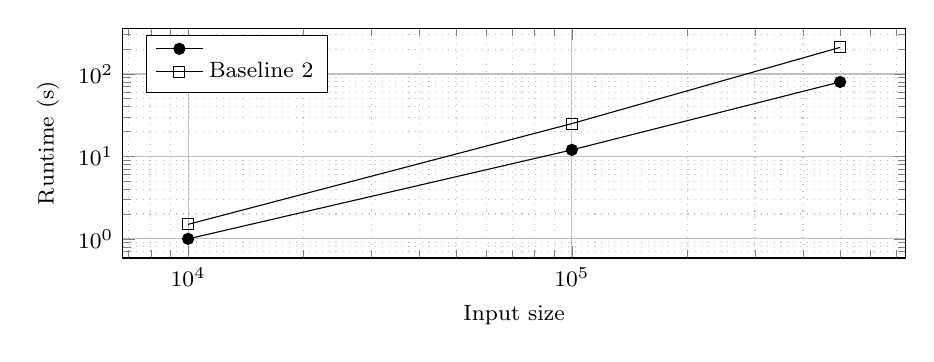
\begin{tikzpicture}
        \begin{loglogaxis}[
            width=0.95\columnwidth, height=4.5cm,
            xlabel={Input size},
            ylabel={Runtime (s)},
            grid=both, minor grid style={dotted},
            legend pos=north west, legend cell align=left,
            font=\footnotesize
        ]
        \addplot[mark=*]      coordinates {(1e4,1.0)(1e5,12)(5e5,80)};
        \addlegendentry{\method{}}
        \addplot[mark=square] coordinates {(1e4,1.5)(1e5,25)(5e5,210)};
        \addlegendentry{Baseline 2}
        \end{loglogaxis}
    \end{tikzpicture}
    \caption{Runtime scaling of \method{}. \method{} scales approximately
    as \(O(n \log n)\), consistent with Section~\ref{sec:method:complexity}.}
    \label{fig:scaling}
\end{figure}

\subsection{Sensitivity to Hyperparameters}
\label{sec:experiments:sensitivity}

\textbf{[Optional --- include if your method has hyperparameters whose
sensitivity matters.]} We sweep the regularization weight \(\lambda\)
from \(10^{-3}\) to \(10^{1}\). \method{} is stable across two orders
of magnitude, with the best results at \(\lambda = \textbf{[value]}\).
The full sweep is reported in the supplementary material.

\subsection{Case Study}
\label{sec:experiments:case}

\textbf{[Optional but recommended for journals --- pick one concrete,
realistic instance and walk through it in depth.]} We present a case
study on \textbf{[specific design / problem instance]} to demonstrate
the practical applicability of \method{}. Compared to the default
baseline, \method{} \textbf{[concrete improvement on this instance]}.
